% !TeX spellcheck = de_CH_frami
\newpage
\section{Einstufige MOS-Verstärker (Kap. 10)}
Grosssignal-Analyse (Arbeitspunktberechnung), Kleinsignal-Analyse (Signalberechnung)\\
\textbf{Tipp:} Jede Gate-Drain Strecke invertiert das Vorzeichen der Kleinsignalübertragung.\\
\begin{tabular}{|p{0.16\textwidth}p{0.44\textwidth}|p{0.3\textwidth}|}
	\hline
	\textbf{Verstärker mit Widerstandslast}&\textbf{Kleinsignal Ersatzschaltung}&\textbf{Verstärker mit MOS-Dioden-Last}\\
	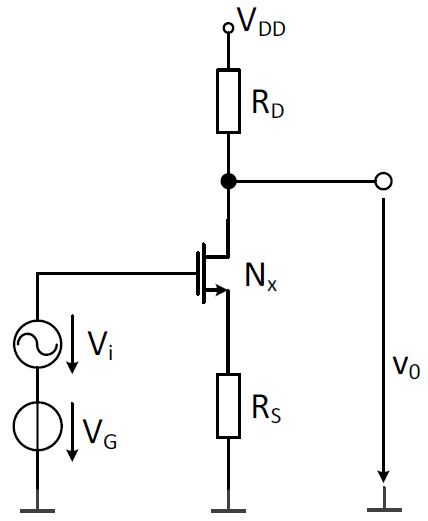
\includegraphics[height=3.5cm]{chapters/Verstaerker/images/AmpWiderstand}&
	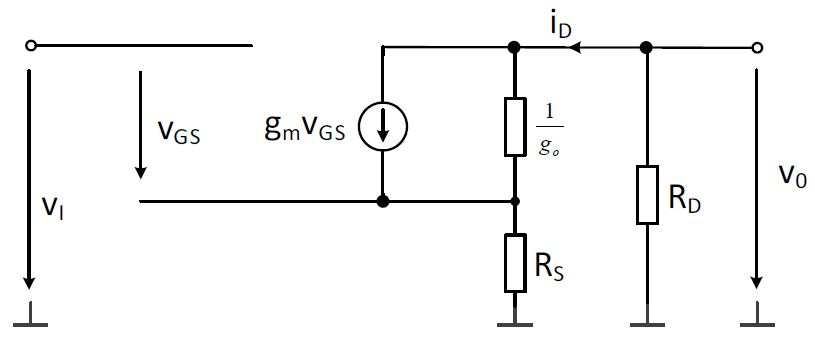
\includegraphics[height=3.5cm]{chapters/Verstaerker/images/AmpWiderstandKS}&
	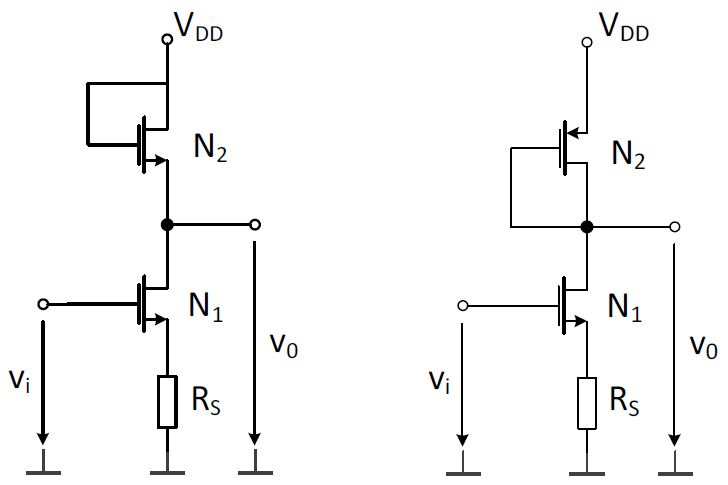
\includegraphics[height=3.5cm]{chapters/Verstaerker/images/AmpDiode}\\ 
\end{tabular}\\
\begin{tabular}{|p{0.18\textwidth}p{0.2\textwidth}|p{0.25\textwidth}|p{0.245\textwidth}|}
	\hline
	\textbf{Verstärker mit Stromquellenlast}&\textbf{Realisierung}&\textbf{Verstärker mit parallelem Eingang (Push-Pull)}&\textbf{Verstärker mit Stromumlenkung}\\
	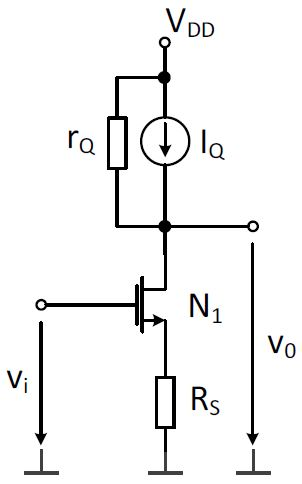
\includegraphics[height=3.5cm]{chapters/Verstaerker/images/AmpStromquelle}&
	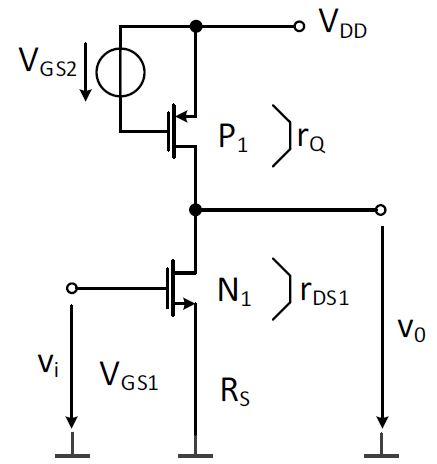
\includegraphics[height=3.5cm]{chapters/Verstaerker/images/AmpStromquelleReal}&
	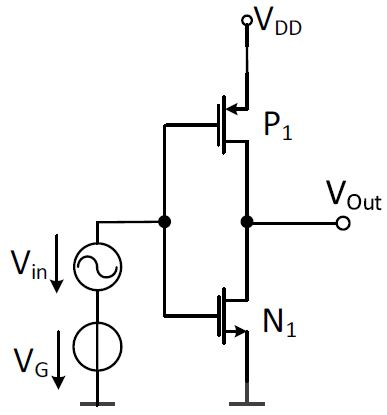
\includegraphics[height=3.5cm]{chapters/Verstaerker/images/AmpPushPull}&
	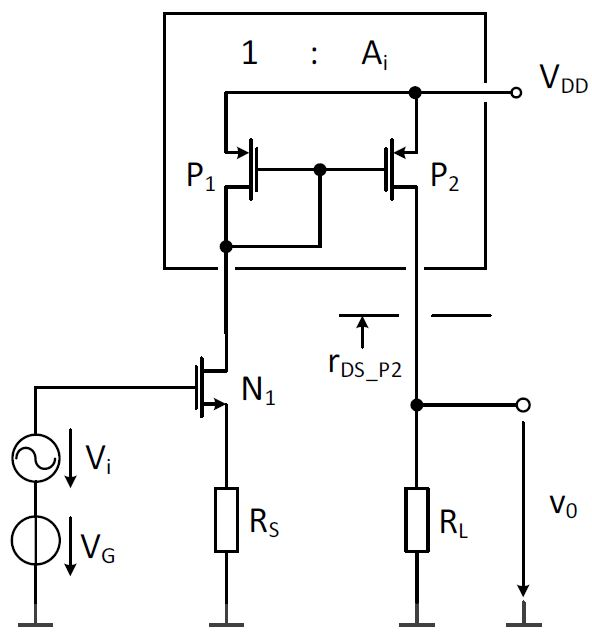
\includegraphics[height=3.5cm]{chapters/Verstaerker/images/AmpStromumlenkungR}
\end{tabular}\\
\begin{tabular}{|p{0.3\textwidth}|p{0.3\textwidth}|p{0.3\textwidth}|}
	\hline
	\textbf{Kaskode mit Widerstandslast}&\textbf{Kaskode mit Stromquellenlast}&\textbf{Gefaltete Kaskode}\\
	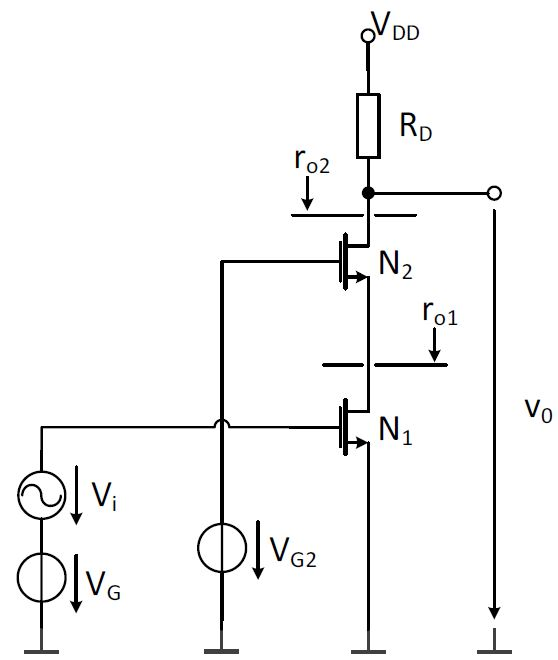
\includegraphics[height=3.5cm]{chapters/Verstaerker/images/AmpKaskodeR}&
	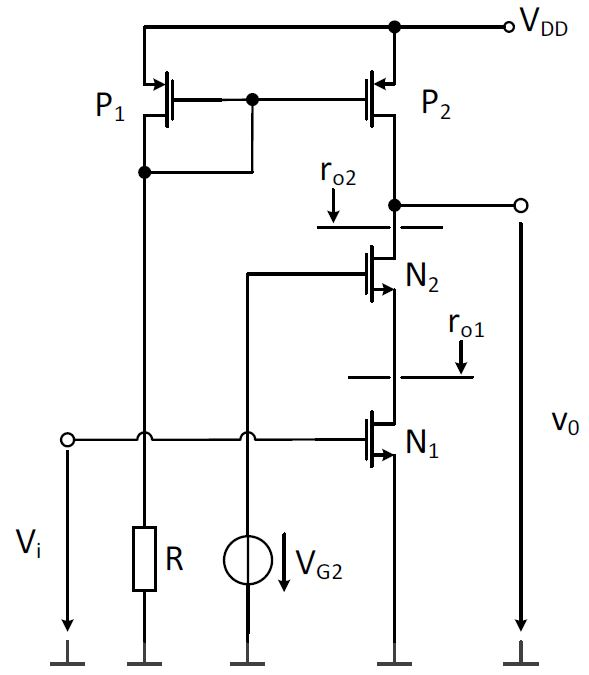
\includegraphics[height=3.5cm]{chapters/Verstaerker/images/AmpKaskodeIq}&
	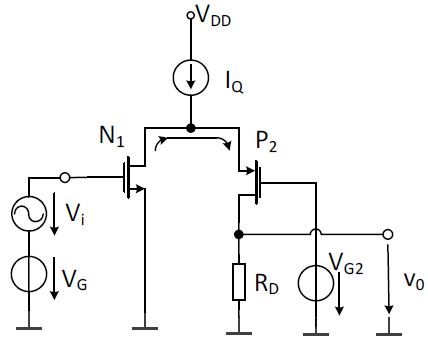
\includegraphics[height=3.5cm]{chapters/Verstaerker/images/AmpFoldedKaskode}\\ \hline
\end{tabular}\\
\begin{tabular}{|l|l|}
	\hline
	Verstärker mit Widerstandslast&$a=-\frac{g_m}{\frac{1}{R_D}+g_0}$\\
	&$r_{out}=r_{iD}=\frac{1}{g_0}(1+g_mR_S)+R_S$\\ \hline
	Verstärker mit MOS-Dioden-Last&$a=-\frac{\frac{1}{g_{m2}}}{R_S+\frac{1}{g_{m1}}}\textcolor{gray}{=-\frac{g_{m1}}{g_{m2}}=-\sqrt{\frac{\beta_1}{\beta_2}}}$ \textcolor{gray}{(wenn $R_S = 0$)}\\ \hline
	Verstärkung mit Stromquellenlast&$a=-\frac{R_D}{R_S+\frac{1}{g_m}+(R_D+R_S)\frac{g_o}{g_m}} \textcolor{gray}{=-\frac{g_{m1}}{\frac{1}{r_Q}+g_{o1}}}$\\ \hline
	Verstärker mit parallelem Eingang (Push-Pull-Stufe)&$a=-\frac{g_{m\_N1}+g_{m\_P1}}{g_{o\_N1}+g_{o\_P1}}= -(g_{m\_N1}+g_{m\_P1})\cdot (r_{DS\_N1}||r_{DS\_P1})$\\ \hline
	Verstärker mit Stromumlenkung&$a\approx a_i\frac{R_L||r_{DS3}}{R_S+r_{S1}}$\\ \hline
	Kaskode mit Widerstandslast&$a\approx -g_{m1}R_D$\\ \hline
	Kaskode mit Stromquellenlast&$a \approx -\frac{g_{m1}}{g_{o3}}$ \\ \hline
\end{tabular}